% Dette er utf8 udgaven af latex-templaten. Den er til brug på
% systemer der kører utf8x, såsom linux. Hvis du bruger windows, så er
% det letteste at hente windowsudgaven i stedet, da den i forvejen er
% gemt i latin1 format og har dette sat i inputenc. Hvis du ikke
% benytter danske tegn (æ,ø,å), så er det lige meget.
% 
% Loader dokumentklassen memoir. Sætter sproget i dokumentet til
% dansk, papirtypen til A4, sætter dokument til lige store højre og
% venstre margen, laver to søjler og siger at vi gerne vil lave en
% artikel, sætter skriftstørrelse til 9pt.
\documentclass[danish,a4paper,twoside, 11pt]{memoir}
%\setsecnumdepth{subsection}
\settocdepth{subsection}

\usepackage[danish]{babel} %Giver mulighed for dansk orddeling. Slet
% kun hvis du VED hvad du laver, eller skal
% skrive noget på engelsk.
\usepackage[utf8x]{inputenx} %Hvis du benytter windows i stedet for
% linux, så skift utf8 ud med
% latin1. Tillader danske tegn.
\usepackage{graphicx} %Tillader indsættelse af billeder
\usepackage{caption}
\usepackage{mathtools} %Ekstra matematik... bare lad den være, du får
% muligvis brug for den.
\usepackage{siunitx} %Bruges til at indsætte SI enheder med
% makroer. Sørger for at de kommer til at stå med
% rigtig skrifttype (normal skrift i
% matematik). Brug den, eller lad være. ²
% indsættes med \squaren for at undgå sammenfald
% med \square fra ams.
% \usepackage{url} %bruges til at formattere url'er... kan sagtens udelades.
\usepackage[version=3]{mhchem}
%\usepackage[hidelinks=true]{hyperref}
\usepackage{microtype} % Pakke der proever at fikse badbox
% problemer. Kun kompatibel med pdflatex.


\usepackage{suffix}
\usepackage{wasysym}
\usepackage{multirow}
\usepackage{xspace}
\usepackage[caption=false]{subfig}
\let\subbottom\subfloat

\usepackage[flushleft]{threeparttable}
\usepackage[draft]{fixme}
\renewcommand\fxdanishfatalname{Fatal}

\usepackage[square,sort,comma,numbers]{natbib}


%%%% Forside stuff
\usepackage{mathpazo}% palatino + matematik
\usepackage{bm}
\usepackage{soul} % lege lege

%\usepackage{autonum}
\usepackage[hidelinks]{hyperref}
\usepackage{cleveref}



%%%%%%%%%%%%%%%%%%%%%%%%%%%%%%%%%%%%%%%%%%%%%%%%%%%%%%%%%%%%%%%%%%% 
%%%%%%%%%%%%%%%%%%%%%%          Forside          %%%%%%%%%%%%%%%%%%
%%%%%%%%%%%%%%%%%%%%%%%%%%%%%%%%%%%%%%%%%%%%%%%%%%%%%%%%%%%%%%%%%%%

\sodef\an{}{0.2em}{.9em plus.6em}{1em plus.1em minus.1em}
\newcommand\stext[1]{\an{\scshape#1}}
\pagestyle{simple} %Giver tom footer og sidetal i header
\usepackage{calc}
\newif\ifNoChapNumber
\makeatletter
\makechapterstyle{VZ34}{
  \setlength{\beforechapskip}{0.1pt}
  \setlength{\midchapskip}{1.0\onelineskip}
  \setlength{\afterchapskip}{1.5\onelineskip}
  \renewcommand\chapternamenum{}
  \renewcommand\printchaptername{}
  \renewcommand\printchapternum{}
  \renewcommand\chapnumfont{\Huge\bfseries}
  \renewcommand\chaptitlefont{\Huge\bfseries\raggedright}
  \renewcommand\printchaptertitle[1]{%
    \begin{tabular}{@{}p{1cm}|!{\quad}p{\textwidth-1cm-2em-4\tabcolsep }}
      \ifNoChapNumber\relax\else\chapnumfont \thechapter\fi
      & \chaptitlefont ##1
    \end{tabular}
    \NoChapNumberfalse
  }
  \renewcommand\printchapternonum{\NoChapNumbertrue}
}
\chapterstyle{VZ34}
%\chapterstyle{tandh}

%%%%%%%%%%%%%%%%%%%%%%%%%%%%%%%%%%%%%%%%%%%%%%%%%%%%%%%%%%%%%%%%%%%
%%%%%%%%%%%%%%%%%%%%%% Costumized math functions %%%%%%%%%%%%%%%%%%
%%%%%%%%%%%%%%%%%%%%%%%%%%%%%%%%%%%%%%%%%%%%%%%%%%%%%%%%%%%%%%%%%%%

\renewcommand{\d}[2]{\frac{d #1}{d #2}} % for derivatives
\newcommand{\dd}[2]{\frac{d^2 #1}{d #2^2}} % for double derivatives
\newcommand{\pd}[2]{\frac{\partial #1}{\partial #2}} 
% for partial derivatives
\newcommand{\pdd}[2]{\frac{\partial^2 #1}{\partial #2^2}} 
% for double partial derivatives
\newcommand{\pddd}[2]{\frac{\partial^3 #1}{\partial #2^3}}
\newcommand{\mvec}[1]{\bm{#1}}

\graphicspath{{./Figures/}}
\setkeys{Gin}{width=0.9\columnwidth}



%%% Grundstoffer
\newcommand{\Pu}{\ce{^{239}Pu}\xspace}

%Be-8
\newcommand\Be{\ce{^{8}Be}\xspace}
\WithSuffix\newcommand\Be*{\ce{^{8}Be^*}\xspace}
% C-12
\newcommand\Carb{\ce{^{12}C}\xspace}
\WithSuffix\newcommand\Carb*{\ce{^{12}C^*}\xspace}

%%% Siunitx
\sisetup{separate-uncertainty=true,
  quotient-mode = fraction,
  free-standing-units = true,
  use-xspace = true,
  space-before-unit = true}

\DeclareSIUnit\um{\micro\meter}
\DeclareSIUnit\MV{\mega\V}
\DeclareSIUnit\ub{\micro\barn}


%%%% Små ord
\newcommand{\beamline}{strålerøret\xspace}
\newcommand{\target}{strålemål\xspace}
\newcommand{\lAND}{\texttt{OG}\xspace}
\newcommand{\lOR}{\texttt{ELLER}\xspace}




%%%%%%%%%%%%%%%%%%%%%%%%%%%%%%%%%%%%%%%%%%%%%%%%%%%%%%%%%%%%%%%%
%%%%%%%%%%%%%%%%%% Header setup %%%%%%%%%%%%%%%%%%%%%%%%%%%%%%%% 
%%%%%%%%%%%%%%%%%%%%%%%%%%%%%%%%%%%%%%%%%%%%%%%%%%%%%%%%%%%%%%%% 



\begin{document}


\begin{titlingpage}
  \thispagestyle{empty}
  \centering
  { \setlength{\baselineskip}{24pt}
    {\Huge \stext{Carbon-12's} \par
      %\textit{for}\par
      \stext{henfaldsprocess}
    }\par
    \stext{(The decay process of carbon-12)}
    \par\vspace*{4\onelineskip}
    \par
    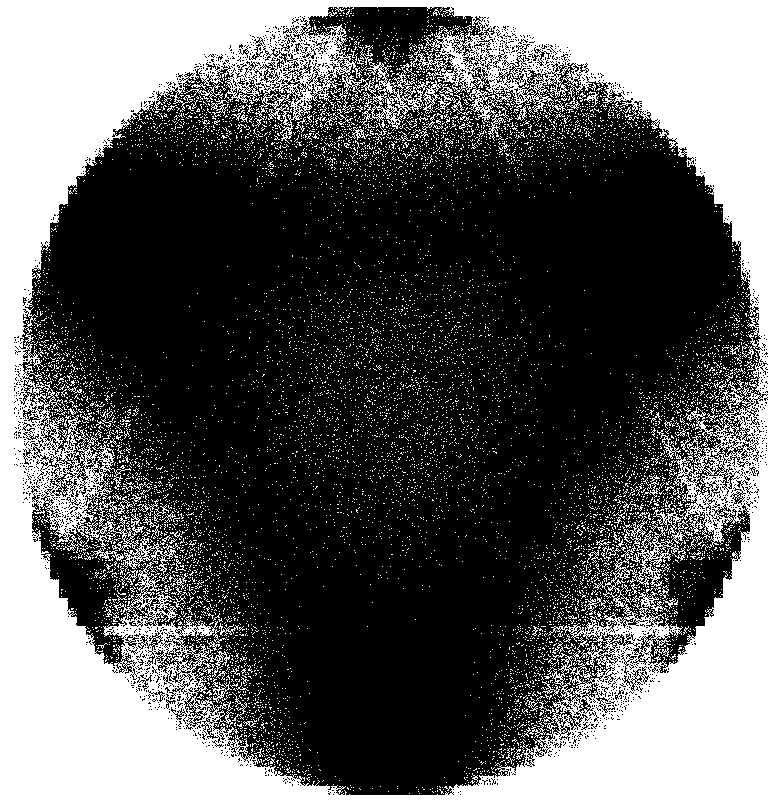
\includegraphics[width=8cm]{forside} 
    \par\vspace*{5\onelineskip}
    \stext{Bachelorprojekt i Fysik}\par
    \large\stext{Michael Kulmback Munch \par 20103561}\par
  }
  \vfill
  \vspace*{2\onelineskip}
  \stext{Vejleder: Hans Fynbo}\hfill
  \stext{1. juli 2013}
  \par\vspace*{2\onelineskip}
  \small
  \stext{Institut for Fysik og Astronomi}\par
  \stext{Aarhus Universitet}
  \enlargethispage{2\onelineskip}

  \newpage
  \thispagestyle{empty} % fjerne evt. sidehoved og -fod
  \small
  % resten af teksten indenfor dette env skal være \small
  \strut\vfill  % pres alt ned i bunden af siden
  \begin{flushleft}
    Institut for Fysik og Astronomi \par
    Aarhus Universitet \par
    Ny Munkegade, Bygning 1520 \par
    DK-8000 Aarhus C \par
    Danmark \par
    \vspace{\onelineskip}
    
    \copyright\ Michael Munch 2013                      \par
    \fxfatal{Not done yet}
    Forsidebilledet er et Dalitzplot.
  \end{flushleft}
\end{titlingpage}
%\cleardoublepage
\thispagestyle{empty} % ingen sidehoved eller -fod
\vspace*{\stretch{3}} % speciel faktoriseret gummilængde
\begin{center}
Tak til Hans og Kasper for deres tålmodighed.
\end{center}
\vspace*{\stretch{17}}
% ting efter siden skal starte på en højre side
\cleardoublepage
     
\frontmatter

\tableofcontents
\newpage
\listoffixmes

\mainmatter
\chapter{Indledning}
\label{cha:indledning}
\vspace{-0.5\onelineskip}

På baggrund af en stribe artikler udgivet af Cockcroft og Walton fra 1930 og fremefter \cite{Walton}
beskrev Oliphant og Rutherford i deres artikel, "Transmutations of Elements by Protons"{} fra 1933
\cite{Rutherford}, deres udkast til en forbedret partikelaccelerator. Disse acceleratorer muliggjorde
udforskning af nye områder inden for kernefysikken, da det var muligt at opnå intensiteter svarende
til 180\gram rent radium, hvilket tidligere havde været en af de primære kilder til energirige
partikler.

I denne artikel studerer Oliphant og Rutherford bl.a. spredning af protoner på \Bor og ud fra en
simpel model viser de, at de eksperimentelle data er i overenstemmelse med, at \Carb henfalder til
tre $\alpha$-partikler. Deres eksperimentelle data er ikke følsomme over for den specifikke
henfaldsproces, hvilket de selv påpeger. 

Forståelse af denne proces er relevant, da den giver information om trippel-$\alpha$ processen
$3\alpha\rightarrow\Carb$ i stjerner. Kort sagt kan \Carb henfalde enten direkte til tre $\alpha$-partikler
eller via en tilstand i \Be. Dette kræver præcisionsmålinger, der ikke var mulige med datidens
eksperimentelle udstyr. Udvikling inden for faststoffysik gav nye detektortyper, som tillod at måle
energien med større præcision. Disse detektorer udspænder kun en lille rumvinkel, så det er
nødvendigt at benytte flere detektorer og at flytte disse rundt for at opnå stor dækning. Dette er en
meget tidskrævende proces. Denne viden kan også benyttes til mere jordnære formål, da $p+\Bor
\rightarrow \Carb$ er en mulig kandidat til en fusionproces, der ikke frigiver neutroner. 

Den opstilling, som benyttes her i projektet, er en del af LOBENA-projektet. Her benyttes i stedet
store segmenterede faststofdetektorer, hvilket muliggør detektion af energi og position samtidig med,
at en stor rumvinkel dækkes. Formålet med LOBENA er at studere kernestrukturen af \Be, \Carb og
\ce{^{16}O} ved at populere tilstande i disse grundstoffer og studere henfaldsprodukterne. Her søges
bl.a. efter en $2^{+}$ resonans i \Carb, som blev forudsagt i 1956, men det er stadig ikke afgjort,
om denne eksisterer.

Jeg blev tilknyttet projektet, da disse detektorer lige var blevet installeret og denne rapport vil
derfor først omhandle processen med at forstå opbygningen af detektorerne med henblik på at foretage
en kalibrering. Kalibreringen benyttes i analysen af de eksperimentelle data for \Carb til at
bestemme $\alpha$-spektret og såkaldte Dalitzplot, der grafisk illustrerer systemets vekselvirkninger. På
baggrund af disse argumenteres for henfaldsprocessen af \Carb.

Rapporten starter med en beskrivelse af den eksperimentelle opstilling og det eksperimentelle og
analytiske arbejde. Dernæst følger et kapitel, hvor kalibreringen af udstyret gennemgåes. I det
følgende kapitel verificeres kalibreringen. Til sidst kommer analysen af de eksperimentelle
resultater.







\chapter{Opstilling}
\label{cha:opstilling}

Et beam af protoner accelereres op til den ønskede energi med en 5\MeV Van de Graaf
accelerator. Dette beam afbøjes med en eletromagnet og sendes ind i beamline, hvor det først
passerer gennem et hul i midten af den ene detektor, hvorefter en del af det vil kolliderer med et
\ce{^{11}B}-target på carbon backing.
\fxfatal{Hvad er tykkelsen af foliet og backing?}
Det resterende vil passere videre gennem beamline, hvor det
igen vil passere gennem en detektor, for at ende i en Faraday cup.

Detektorsystemet består af to dobbel siddet silicium strip detektorer (DSSSD), som fungerer på samme
måde, som almindelige fasstofdetektorer. Fordelen er opdelingen af forsiden og bagsiden i et antal
områder kaldet strips. Dermed er det muligt at bestemme både vinkel og energi af
partiklerne. Bagsiden er opdelt i 32 radiale slices, som benævnes sektorer. Forsiden er derimod
opdelt i en række ringe, der hver er 886\um tykke, med et 100\um isolerende område mellem hver.

Den første detektor beamet passerer igennem kaldes upstream. Denne udspænder vinklerne fra
$141\degree$ til $165\degree$ målt fra beamets retning. Den anden benævnes med downstream og den
udspænder fra $15\degree$ til $40\degree$.


\begin{figure}[h]
  \centering
  \fxfatal{Skematisk tegning af opstillingen mangler.}
  %\includegraphics{}
  \caption{Skematisk tegning af opstillingen}
  \label{fig:opstilling}
\end{figure}

\chapter{Det eksperimentelle arbejde}
\label{cha:eksp}


\chapter{Kalibrering}
\label{cha:kalibrering}

\chapter{Rutherford}
\label{cha:rutherford}

\chapter{Henfaldprocessen af \Carb}
\label{cha:sekventielt-henfald}
I dette afsnit præsenteres den sekventielle henfaldsmodel, hvorefter der foretages kinematiske
beregninger, der illustrerer hvilket energispektrum dette vil give anledning til. Dette efterfølges
af eksperimentelle resultater, der benyttes til at afgøre om henfaldet foregår ved denne proces.  

\section{Teoretisk baggrund}
\label{sec:sekventiel-teo}

For et henfald, hvor moderkernen deles i to, et såkaldt to-partikelhenfald {$M \rightarrow a + b$},
er der otte frihedsgrader - to impulsvektorer, hver med tre komponenter, samt to energier. Disse
størrelser er underlagt bevarelseslovene for energi og impuls, hvilket reducerer antallet af
frihedsgrader til nul. I et energispektrum vil et sådant henfald give anledning til to
toppe. Energierne af disse i massemidtpunktssystemet for moderkernen er givet ved
\begin{equation}
  \label{eq:toE}
  T_{a} = \frac{m_{b}}{m_{a} + m_{b}}Q, \qquad T_{b} = \frac{m_{a}}{m_{a} + m_{b}}Q.
\end{equation}

Tre-partikelhenfaldet, {$M \rightarrow a + b + c$}, har derimod 12 frihedsgrader - ni fra impuls og
tre fra energi. Dette kan reduceres ved at overveje følgende; henfaldet foregår i ét plan, så
$p_{i,z}$ kan sættes lig nul. Dette fjerner tre frihedsgrader. Energi- og impulsbevarelse eliminerer
tilsammen tre frihedsgrader. Energi-impuls relationen, $E^{2} = p^{2} + m^{2}$, anvendt for hver
enkelt datterkerne begrænser også tre frihedsgrader. En rotation i xy-planet ændrer ikke systemet,
hvilket fjerner én enkelt frihedsgrad. Antallet af frihedsgrader kan dermed reduceres til to,
hvilket betyder, at systemets tilstand afgøres af dynamikken, dvs. vekselvirkninger i systemet.

Henfalder \Carb-kernen direkte til tre ikke-vekselvirkende $\alpha$-partikler, vil energispektret
pga. de to frihedsgrader udgøre et kontinuum af energier. Denne proces kaldes direkte henfald og
er skitseret på \cref{fig:becker}a.

\begin{figure}
  \centering
  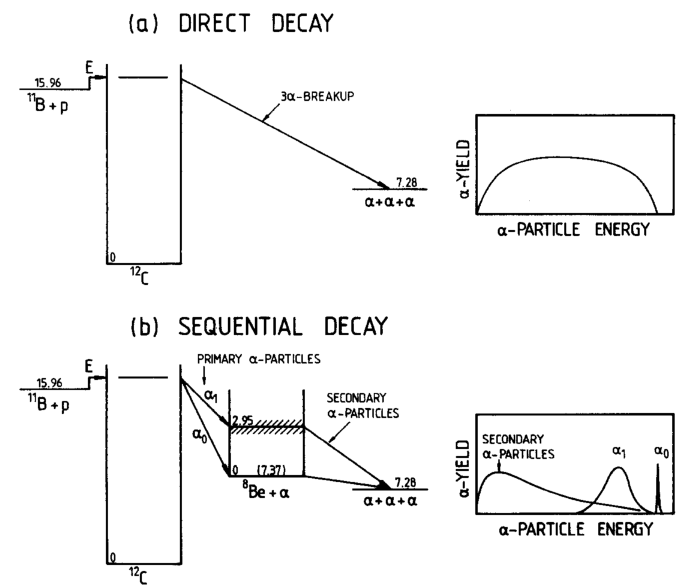
\includegraphics{Becker}
  \caption{Energidiagram for henfaldsprocessen af \Carb skitseret for hhv. (a) direkte henfald  og
    (b) sekventielt henfald. Figuren er lånt fra \cite{becker}.}
  \label{fig:becker}
  \vspace{-5mm}
\end{figure}

\subsection{Sekventielt henfald}
\label{sec:sekventielt-henfald}

End anden mulighed for tre partikel henfald er to på hinanden følgende to partikel henfald. Dette
kaldes for sekventielt henfald. I tilfældet med \Carb henfalder den først til en tilstand i \Be
under udsendelse af en $\alpha$-partikel. Modsat det direkte henfalder, som neglicerer vekselvirkninger
mellem henfaldprodukterne, så svarer dette til en kraftig vekselvirkning med to af de tre
$\alpha$-kerner. Beryllium kernen vil derefter henfalde til to sekundære $\alpha$-partikler. 

Antallet af frihedsgrader er det samme som for det direkte henfald, hvilket virker mærkeligt, da der
blot er tale om to to partikel henfald, hvor antallet af frihedesgrader er nul. Dette skyldes, at
det ikke er muligt at befinde sig i CM for begge de to henfald. Det sekventielle henfald vil derfor
både give anledning til toppe og et kontinium. .

% Med sekventielt henfald menes henfald fra den populerede tilstand i \Carb først med et primært
% henfald \Be samt en $\alpha$-partikel, hvor beryllium kernen foretager et sekundært henfald til to
% $\alpha$-partikler. Dette vil give andledning til et anderledes spektrum end et direkte henfald fra \Carb
% til tre $\alpha$-partikler, som giver andledning til et kontinium af tilstande, der afgøres af vinklen
% mellem de enkelte $\alpha$-partikler, se \cite{Becker}.

Den sekventielle henfaldsproces er illustreret på \cref{fig:becker}b, og tages udgangs i CM for
moderkernen, så vil det sekventielle henfald af \Carb give anledning til en smal top ved energien
svarende til henfald grundtilstanden af \Be.
\begin{equation}
  \label{eq:alpha0}
  \Carb* \rightarrow \Be(0^{+}) + \alpha_{0} \rightarrow 2\alpha_{2} + \alpha_{0}
\end{equation}
På trods af at beryllium-8 er ustabil er grundtilstanden stadig ret smal med en bredde på kun
\SI{6.8}{\eV}. Derfor vil bredden af toppen primært skyldes detektorens opløsningsevne. 

Ved de protonenergier, der arbejdes med, så er der endvidere mulighed for at henfalde til den første
exiterede tilstand i \Be, der ligger \SI{2.95}{\MeV} over grundtilstanden.
\begin{equation}
  \label{eq:alpha0}
  \Carb* \rightarrow \Be*(2^{+}) + \alpha_{1} \rightarrow 2\alpha_{2} + \alpha_{1}
\end{equation}
Bredden af denne top afgøres primært af bredden af beryllium tilstanden, som er
\SI{1.5}{\MeV}. Toppen vil derfor stort set svare til en Breit-Wigner fordeling, der er væsenlig
breddere, samt ligger ved lavere energi end den for $\alpha_{0}$.

Idet begge berylliumtilstande er ustabile vil der, pga. den korte levetid, forekomme endnu et
henfald udmiddelbart efter. Dette vil give andledning de to sekundære $\alpha$-partikler hhv.
$\alpha_{21}$ og $\alpha_{22}$. Energien af disse kan bestemmes ud fra følgende kinematiske overvejelser.

\subsubsection{Kinematik}
\label{sec:sekv-kinematik}

En skitse af situationen efter det sekundære henfald ses på \cref{fig:secundary}.
\begin{figure}[h]
  \centering
  \includegraphics[width=0.6\columnwidth]{Sekventiel-kinematik}
  \caption{Skitse af situationen af det sekundære henfald. Vektorerne angiver hastighederne. $\phi$ er
    vinklen mellem hastigheden af beryllium og de sekundære $\alpha$-partikler i CM for beryllium. $\phi_{2i}$ er
    de tilsvarende vinkler i LAB-systemet.}
  \label{fig:secundary}
\end{figure}

Både i laboratorie- (LAB) og massemidtpunktsystemet (CM) følger af energi og impulsbevarelse,
at energien af de to primære henfaldsprodukter må være
\begin{equation}
  \label{eq:Ealpha0}
  E_{\alpha_{0}} = \frac{2}{3} Q_{1} \qquad E_{\ce{Be}} = \frac{1}{3} Q_{1},
\end{equation}
hvor $Q_{1}$ er den frigivne energi ved det primære henfald $\Carb \rightarrow \alpha + \Be$. Grundet
impulsbevarelse skal de to sekundære $\alpha$'er have lige stor og modsatrettet impuls i CM for
beryllium, Deres hastighed vil danne en vinkel $\phi$ i forhold til beryllium kernens
hastighed. Energien af de to er givet ved
\begin{equation}
  \label{eq:Ealpha2}
  E_{\alpha_{2}}' = \frac{1}{2} Q_{2},
\end{equation}
hvor $Q_{2}$ er den frigivne energi for det sekundære henfald. Hermed ses tydeligt, at i CM er
energien af de sekundære partikler konstant uanset vinklen.

De tilsvarende størrelser i LAB systemet kan bestemmes ved at tage højde for tyngdepunktets
bevægelse, som svarer til berylliumkernens bevægelse
\begin{align}
  E_{\alpha_{2}} %&= \frac{1}{2}m_{\alpha} (\mvec{V_{\ce{Be}}} + \mvec{V_{\alpha}})^{2} \notag \\
  &= \frac{1}{2}m_{\alpha} (V_{\ce{Be}}^{2} + V_{\alpha}^{2} + 2V_{\ce{Be}}V_{\alpha} \cos \phi) \notag \\
  &= \frac{Q_{1}}{6} + \frac{Q_{2}}{2} + \sqrt{\frac{Q_{1}Q_{2}}{3}} \cos \phi,           
  \label{eq:E2LAB} 
\end{align}
hvor der er anvendt approksimationen $m_{\ce{Be}} = 2m_{\alpha}$, og bemærkes at $\phi \leq 0$ for $\alpha_{22}$. 

Ud fra dette ses, at energien af de to sekundære $\alpha$-partikler vil udgøre et kontinium inden for
intervallet $E_{\alpha_{2}} = E_{0} \pm \Delta E$.

For en stråle af protoner med 2\MeV energi, vil henfald til grundtilstanden udgøre energierne mellem
ca. \SI{1.2}{\MeV} og \SI{2.35}{\MeV}, mens henfald til den exciterede tilstand giver andledning til
energier mellem \SI{14}{\keV} og og \SI{5.5}{\MeV}. \fxfatal{Nævn at middelværdien benyttes.}

Den præcise distribution vil afhænge af distributionen af $\cos \phi$, hvilket er bestemt af de populerede
tilstandes impulsmoment. 

Endvidere er det muligt at bestemme vinklen i LAB-systemet ud fra vinklen i CM og Q-værdierne. Dette
kan udledes trigometrisk ud fra \cref{fig:secundary}, men er ikke medtaget her. Resultatet af dette
er
\begin{equation}
  \label{eq:sekv-vinkel}
  \tan \phi_{2i} = \frac{\sin \phi}{\sqrt{\frac{Q_{1}}{3Q_{2}}} \pm \cos \phi}
\end{equation}
Det ses, at som forventet, at den maksimale vinkel fremkommer, når CM-vinklen er 90\degree, svarende
til at al energien tilføres den transversale bevægelse.
\subsection{Dalitzplottet}
\label{sec:dalitz}

Som nævnt i starten af kapitlet afhænger energien af datterkernerne i tre-partikelhenfaldet af
dynamikken i systemet. Derfor indføres Dalitzplottet, som grafisk illustrerer dynamikken.

\subsubsection{Teoretisk baggrund}
\label{sec:dalitz-teori}


Fermis gyldne regel angiver raten af et givent henfald \cite[s. 16]{Bettini}
\begin{equation}
  \label{eq:fermi}
  W = 2\pi|M_{fi}|^{2}\rho,
\end{equation}
hvor $\rho$ er tilstandstætheden eller faserumsvolumen af sluttilstanden. $M_{fi}$ kaldes
matrixelementet og er et mål for koblingen mellem start- og sluttilstanden. Ser man bort fra den
rumlige orientering og udnytter, at $T_{1} + T_{2} + T_{3} = Q$, kan sluttilstanden beskrives ved
kun to variable $T_{1}$ og $T_{2}$. Med denne begrænsning er det muligt at vise følgende for
henfaldssandsynligheden $\zeta$ \cite{Kallen}
\begin{equation}
  \label{eq:DOS}
  \frac{d\zeta}{dT_{1}dT_{2}} \propto |M_{fi}|^{2}.
\end{equation}
Sandsynlighedsfordelingen af $\zeta$ i forhold til de kinetiske energier er dermed et direkte mål for
kvadratet af matrixelementet. 

Idet henfaldssandsynligheden er proportional med antal henfald, kan denne visualiseres grafisk. Et
godt valg af koordinater kan findes, hvis man tager udgangspunkt i, at sluttilstanden af systemet
består af tre ens partikler. Dette kan udnyttes ved at benytte den geometriske egenskab ved en
ligesidet trekant; den vinkelrette afstand fra siderne til givent et punkt er lig højden. Denne
egenskab kendes også som Vivianis sætning.

\Cref{eq:dalitz} viser et sæt af koordinater, for hvilke disse afstande er proportionale med de
kinetiske energier
\begin{equation}
  \label{eq:dalitz}
  x = \frac{T_{1}+2T_{2}}{Q\sqrt{3}}, \hspace{3cm} y = \frac{T_{1}}{Q} - \frac{1}{3}.
\end{equation}
Heraf følger, at punkterne svarende til trippel $\alpha$-henfald vil ligge inden for trekanten grundet
energibevarelse. Endvidere kan det vises \cite{dalitz}, at impulsbevarelse begrænser punkterne til
trekantens indskrevne cirkel. Dette er illustreret på \cref{fig:dalitz-triangle}a. Denne type plot
kaldes et Dalitzplot.

\begin{figure}[h]
  \centering
  \subbottom[Dalitzplottet givet ved koordinaterne i \cref{eq:dalitz}. Trekanten svarer til
  energibevarelse og cirklen til impulsbevarelse.]
  {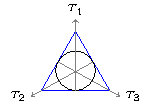
\includegraphics[width=0.48\columnwidth]{dalitz-tri}}
  % 
  \hfill
  % 
  \subbottom[Dalitzplottet med indtegnede resonansbånd. Det smalle røde viser $\alpha_{0}$, mens den bredde
  viser $\alpha_{1}$.]
  {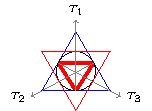
\includegraphics[width=0.48\columnwidth]{dalitz-band}}%
  \caption{}
  \label{fig:dalitz-triangle}
\end{figure}

\subsubsection{Symmetribetragtninger}
\label{sec:symbetragt}

Såfremt der ikke er nogen symmetribegrænsninger og henfaldsprodukterne ikke vekselvirker med
hinanden, vil matrixelementet være en konstant og henfaldet vil udelukkende afgøres af
faserummet. Dette svarer til statistisk henfald og vil give anledning til en flad fordeling
\cite{Fedorov}, hvilket vil være tilfældet ved direkte henfald.

Henfalder systemet i stedet via en resonans for derefter at henfalde til sluttilstanden, vil det ses
på plottet som et bånd. I forhold til den sekventielle henfaldsmodel og koincidensspektrene
forventes bånd svarende til energien af $\alpha_{0}$ og $\alpha_{1}$. Bredden af disse bånd vil være bestemt
af berylliumtilstandens bredde. $\alpha_{1}$-båndet bør derfor være væsentligt breddere, hvilket er
indtegnet på \cref{fig:dalitz-triangle}b. Dalitzplottet kan dermed bruges til at identificere
resonanser og bredden af disse.

$\alpha$-henfaldet er ikke et svagt henfald, så både spin og paritet skal være bevaret. Endvidere er
$\alpha$-partikler bosoner, så den samlede bølgefunktion skal være symmetrisk under ombytning af de tre
$\alpha$-partikler. På baggrund af disse bevarelseslove skal matrixelementet, og dermed Dalitzplottet,
være nul i visse områder. Denne udledning er foretaget i \cite{Fedorov} og resultatet ses på
\cref{fig:dalitz-0}.
%
\begin{figure}[h]
  \centering
  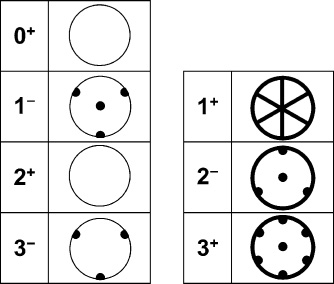
\includegraphics[width=0.3\columnwidth]{dalitz-zero}
  \caption{Områder af Dalitzplottet, hvor fordelingen skal være 0. }
  \label{fig:dalitz-0}
\end{figure}

Den generelle tendens viser, at for tilstandene med unaturlig paritet $\pi = (-1)^{J+1}$, dvs. i højre
kolonne, stiller symmetrien strenge krav til, hvor fordelingen skal være nul. Kravene til
tilstandene med naturlig paritet $\pi = (-1)^{J}$ er væsentligt mindre. Endvidere ses, at det
udelukkende er tilstande med unaturlig paritet, hvor fordelingen skal være nul langs hele randen.

Det er muligt at forklare effekten af $\alpha$-partiklernes bølgenatur på Dalitzplottet mere
intuitivt. Ud fra tre målte energier er der tre mulige måder, hvorpå man kan kombinere de tre
$\alpha$-partikler, således de danner \Be*. Dette svarer til, at der for hver konfiguration er tre
muligheder for hvilken partikel, der udsendes først.

Hvis \Be* tilstanden er smal, er kun en af konfigurationerne realisérbar. Dette svarer til
områderne, hvor $\alpha_{0}$-båndene skærer den indskrevne cirkel på \cref{fig:dalitz-triangle}b. Her er
kun én konfiguration mulig, da den mest energirige partikel nødvendigvis må være
$\alpha_{0}$-partiklen.

% Den første exciterede tilstand i beryllium er dog meget bred, så her vil der være mere end et bidrag
% som summeres. På \cref{fig:dalitz-triangle}b vil det svare til områderne hvor båndene krydser, da
% præcis i disse områder er flere konfigurationsmuligheder.

Den første exciterede tilstand i beryllium er meget bred. I områderne på
\cref{fig:dalitz-triangle}b, hvor $\alpha_{1}$-båndene krydser, vil der være mere end én sandsynlig
konfiguration.  Den endelige bølgefunktion er dermed en linearkombination af flere bølgefunktioner
og idet denne skal være symmetrisk, vil områderne, hvor båndene overlapper, svare til konstruktiv
interferens mellem de enkelte bølgefunktioner. 
















\section{Data og databehandling}
\label{sec:sek-data}
\fxfatal{Snak om program udvikling, ROOT mm.}
\subsection{Koincidens}
\label{sec:koincidens}
For at grovsortere data for protonhændelser var det logiske kredsløb indstillet til \lAND således,
at der kun forekom en hændelse, når to eller flere detektorer blev ramt. Der kan dog stadigvæk
forekomme tilfældige koincidenser i data. Arbejdet bestod derfor i at bestemme de
koincidenser, som svarede til trippel-$\alpha$ henfald.

For at sortere tilfældige fluktuationer i udstyret fra, blev detektioner i forsiden af detektoren
sammenholdt med dem på bagsiden. Idet detektorerne består af et stykke silicium med kontakter på
hhv. for- og bagside, så vil en reel partikel blive detekteret i begge sider. En detektion blev kun
accepteret, hvis der kunne findes en med tilsvarende energi i bagsiden, dog inden for en hvis
tolerance.

\paragraph{Trippelkoincidenser}
\label{sec:trippelkoincidenser}
Hvis der i en given hændelse blev detekteret tre eller flere partikler, blev der ledt efter
trippelkoincidenser. Disse kan forekomme på to måder i detektorerne. Enten vil partiklerne have ramt
hver sin detektor eller også vil to have ramt den samme, mens den tredje rammer en anden
detektor. Hvis den samlede energi af en sådan triplet er lig med Q-værdien, inden for en hvis
tolerance, er det formentlig et sæt af tre matchende $\alpha$-partikler
\begin{equation}
  \label{eq:trippelE}
  T_{1} + T_{2} + T_{3} = Q \pm \Delta E
\end{equation}
Det kritium kan forbedres ved at tage højde for impulsen. Idet detektorerne er positionsfølsomme, er
det muligt at udregne azimut- og polarvinklen af hver partikel. Impulsen kan så udregnes fra
energien $p \propto \sqrt{T}$. For hver triplet udregnes den samlede impuls i CM, hvor den per
konstruktion skal være nul
\begin{equation}
  \label{eq:pCMnul}
  \mvec{p_{1}} + \mvec{p_{2}} + \mvec{p_{3}} = \mvec{0}.
\end{equation}
Ud fra impulsvektorerne er det også muligt at tjekke to andre krav. Er der tale om en sand
koincidens skal summen af vinklerne vektorerne imellem være lig 360\degree. Endvidere foregår
henfaldet i et plan, hvilket matematisk kan formuleres som
\begin{equation}
  \mvec{p_{3}} \cdot (\mvec{p_{1}} \times \mvec{p_{2}}) = \mvec{0}.
\end{equation}

\paragraph{Dobbelkoincidenser}
\label{sec:dobbelkoincidenser}

Hvis spektret er meget rent, er det også muligt at benytte dobbelkoincidenser. Såfremt der kun blev
detekteret to partikler i en hændelse, er de formentlig to tredjedele af en triplet. Energien af den
sidste er derfor differencen mellem Q-værdien og den samlede energi af de detekterede partikler
\begin{equation}
  \label{eq:dobbeltE}
  T_{3} = Q - T_{1} - T_{2}.
\end{equation}

Det er en afvejning, om disse skal medtages. Antallet af detekterede koincidenser øges kraftigt, men
samtidig giver de også anledning til fejl. Nogle åbenlyse fejl kan reduceres ved at tjekke om,
energien af den tredje partikel bliver negativ samt at $x$ og $y$ for Dalitzplottet ligger inden for
den indskrevne cirkel.

Har man udregnet impulsvektorerne for de to detekterede partikler, kan der indføres
et ekstra krav til dobbelkoincidenserne. Den samlede impuls i CM skal være nul. Den ukendte
impuls kan findes ud fra de to detekterede partiklers impuls
\begin{equation}
  \mvec{p_{3}} = -(\mvec{p_{1}} + \mvec{p_{2}}).
\end{equation}
Den kinetiske energi kan også findes ud fra impulsens størrelse, hvilket leder til kravet om, at de to
estimater skal stemme overens
\begin{equation}
  T_{3} = \frac{\lVert\mvec{p_{1}} + \mvec{p_{2}}\rVert^{2}}{2m_{\alpha}}.
\end{equation}

\subsection{Energispektrum}
\label{sec:energispektrum}


\begin{figure}[h!]
  \centering
  \subbottom[Dobbelkoincidenser]{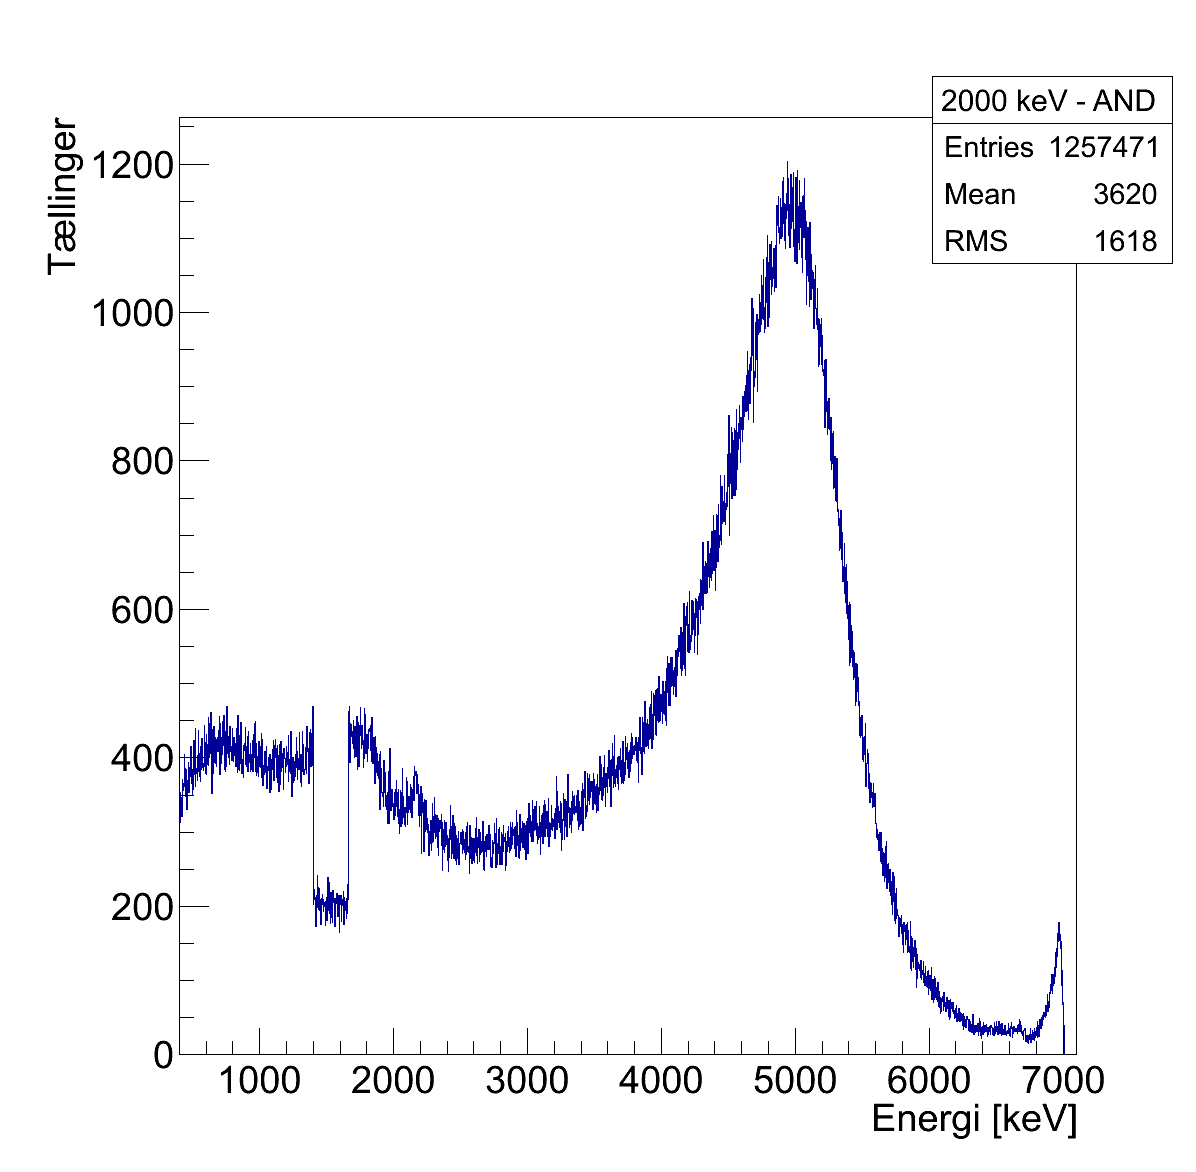
\includegraphics[width=0.46\columnwidth]{1077-spec-D}}%
  \hfill
  \subbottom[Trippelkoincidenser]{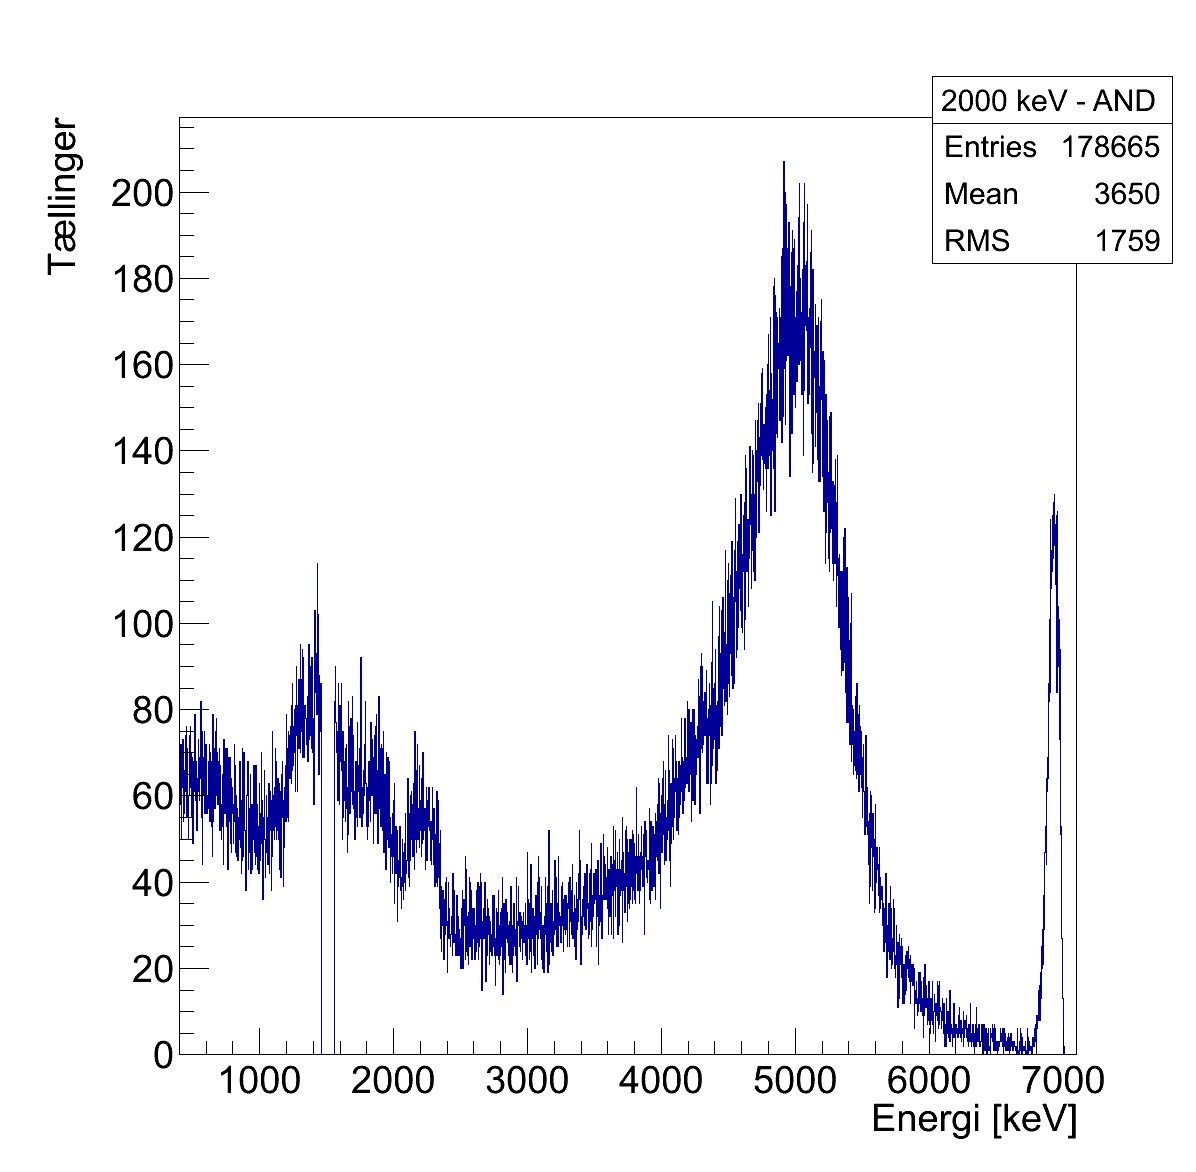
\includegraphics[width=0.46\columnwidth]{1077-spec-T}}%
  \caption{Antal tællinger som funktion af energien for henfald fra \SI{17.8}{\MeV}. Den smalle
    $\alpha_{0}$ og den brede $\alpha_{1}$ top ses tydeligt. Energierne ml. 1400 og 1660\keV er ikke medtaget
    i dobbelkoincidenser. Tilsvarende er 1460 og 1560\keV udeladt for trippelkoincidenserne.}
  \label{fig:alphaSpectrum}
\end{figure}

På \cref{fig:alphaSpectrum} ses alphaspektret i CM for hhv. dobbelt- og trippelkoincidenser, hvor
der er benyttet 2\MeV protoner. Dette populerer en $0^{+}$ tilstand i \Carb med excitations
energi  \SI{17.8}{\MeV}. Idet $\alpha$-henfald bevarer både impulsmoment og paritet, kan henfaldet
foregå både til grundtilstanden og den exciterede tilstand i beryllium. \fxfatal{Flyt til teori
  afsnit og uddyb. Se Hans' tegning. }
\fxfatal{Forklar sammenhæng ml. beamenergien og exitationsenergien af \Carb}

Først og fremmest skal det nævnes, at hvis energien af en af de detekterede $\alpha$-partikler lå mellem
1400 og 1660\keV, så er disse ikke medtaget i dobbelkoincidenserne, da dette gav anledning til
støj. Det samme gør sig gældende for trippelkoincidenserne mellem 1460 og 1560\keV.

I toppen af begge spektrer ses tydeligt en smal top omkring 7\MeV. Under denne ligger der en bred
Breit-Wigner lignende top centreret omkring 5\MeV. Disse toppe stemmer fint overens, både
mht. bredde og energi, med hvad det forventes for $\alpha_{0}$ og $\alpha_{1}$. $\alpha_{1}$-toppen er dog ikke
perfekt Breit-Wigner fordelt, hvilket bla. kan forklares ved, at der forekommer en bidrag fra de 
sekundære partikler.
\fxnote{Fordelingen afhænger også af energien af $\alpha$, som varierer henover toppen. }
Fordelingen af disse er det dog ikke muligt at sige noget videre meningsfuldt
om. Dette skyldes bidrag fra protonstrålen jvf. diskussion i \cref{cha:rutherford}.
\fxfatal{Sørg for at denne reference giver mening.}

De målte spektre er dermed i overenstemmelse med hypotesen om sekventielt henfald til tre
$\alpha$-partikler via \Be. Det essentiele spørgsmål er, om det er muligt at stole på de to
spektre.

Ud fra diskutionen i \cref{sec:sekv-kinematik} især med \cref{eq:Ealpha2} og \cref{eq:sekv-vinkel}
i mente, så ses at energien til rådighed for de sekundære $\alpha$-partikler i den transversale retning
afhænger af Q-værdien af det sekundære henfald.

Et henfald fra grundtilstanden af beryllium til tre $\alpha$-partikler frigører cirka 90\keV, hvorimod et
henfald fra den exciterede tilstand frigører omkring 3\MeV. Dette betyder, at den transversale
komposant af hastigheden af de sekundære $\alpha$-partikler kan være mange gange større, hvilket betyder
at vinklen mellem de to sekundære $\alpha$-partikler kan være tilsvarende større. Benytter man
\cref{eq:sekv-vinkel}, så er den maksimale vinkel hhv. \SI{19}{\degree} og \SI{86}{\degree} for
henfald til grundtilstanden og den exciterede tilstand.

\fxfatal{Dette skal gennemtænkes.}
Med det benyttede dektorsystem er der ikke fuld dækning i alle retninger, men fordi detektorerne er
placeret symmetrisk, så er detektorerne mere effektive til at detektere hændelser med lille vinkel
mellem de sekundære $\alpha$-partikler, da disse to ofte ville ramme samme detektor. Derimod er sandsynligheden
større for at kun to $\alpha$-partikler bliver detekteret, hvis vinklen er større, da der så er mulighed
for at en af partiklerne slet ikke detekteres.

Hvad betyder dette for koincidensspektrene? Effekten er tydeligst ved dobbeltkoincidenserne. Her
undertrykkes $\alpha_{0}$ kraftigst i forhold til $\alpha_{1}$. Dette skyldes, som beskrevet ovenfor, at der
vil være forholdvis flere hændelser, der skyldes henfald til den exciterede tilstand, hvor \emph{kun} to
partikler detekteres. Ved specifik at vælge disse hændelser undertrykkes $\alpha_{0}$-toppen.

Hvorfor er $\alpha_{1}$ så ikke undertrykt i trippelkoincidensspektret? Her er der to effekter, som
spiller ind. For det første er vinklen mellem detektorerne i størrelsesordnen 20\degree, hvilket
betyder, at der er en risiko for at begge sekundære partikler for $\alpha_{0}$ henfaldet rammer ved siden
af. Muligheden for større vinkel ved $\alpha_{1}$ henfald betyder også, at der er mulighed for, at
$\alpha$-partiklerne rammer hver sin detektor. Hvordan disse effekter har indflydelse på spektret er svær
at afgøre, men generelt er sandsynligheden for dektektere $\alpha_{1}$ tripler mindre end den for
$\alpha_{0}$. Forklaringen må af den grund være, at der simpelthen foregår flere
$\alpha_{1}$-henfald. Dette virker umiddelbart mærkeligt idet tunneleringssandsynligheden for
$\alpha$-henfald afhænger kraftigt af energien. Dette er nært relateret til levetiden og et udtrykt for
denne er udledt i \cite[s. 236]{Martin}
\begin{equation}
  \label{eq:SStunnel}
  \lambda \propto w(\alpha) e^{-G}, \qquad G \propto \frac{Z}{\sqrt{E_{\alpha}}}.
\end{equation}
Umiddelbart taler dette også for henfald med $\alpha_{0}$, men faktoren $w(\alpha)$ skal dog bemærkes. Dette
er en "fittefaktor" for at få teorien til at passe med de eksperimentelle data. Faktoren angiver
sandsynlighen for at finde $\alpha$-partiklen inden for kernen. Foltolkningen af
trippelkoincidensspektret er derfor, at det er mere sandsynligt, at $\Carb(\SI{17.8}{\MeV})$ består
beryllium i en $2^{+}$ tilstand sammen med en $L=2$ $\alpha$-partikel, end $0^{+}$ beryllium sammen med
en $L=0$ $\alpha$-partikel. Dette stemmer overens med de tabulerede værdier af tværsnittet i
\cite{States}, der angiver værdierne $\sigma(\alpha_{0}) = \SI{9}{\ub}$ og
$\sigma(\alpha_{1}) = \SI{25}{\ub}$. Værdien for tværsnittet af $\alpha_{1}$-processen er dog mere usikker.

% Dette skyldes at der er tale om
% en vinkeldistribution, som kan antage alle værdier mellem 0 og maksimalværdien. Dermed vil der
% forekomme sekundære partikler fra $\alpha_{1}$ henfald, hvor vinklen er lille. Desuden så er åbningerne
% imellem detektorerne i størrelsesorden 20\degree målt fra \target. Dermed er det muligt at begge
% sekundære partikler fra $\alpha_{0}$ ikke detekteres, hvorimod der er en sandsynlig for at de sekundære
% partikler rammer hver sin detektor, hvis der er tale om $\alpha_{1}$-henfald. Sidst men ikke mindt, skal
% det nævnes, at de sekundære $\alpha$-partikler bidrager til $\alpha_{1}$ toppen. 

Den præcise modulering af de to toppe er dermed meget afhængig hvilke koincidensbetingelser der
stilles, men afhænger også af den specifikke opstilling. For at opnå fuld forståelse af
fordelingen er det derfor nødvendigt at foretage en simulering. Dette ligger dog uden for tidsrammen
af dette projekt. Derfor vil dobbelt- og trippelkoincidenserne behandles separat i den videre
analyse. 



\section{Konklusion}
\label{sec:sekv-konklusion}

I denne afsnit er det vist, at med passende koincidensbetingelser er det muligt at ekstrahere et
samlet energispektrum, som stemmer overens hypotesen om sekventielt henfald.

Desuden er det sandsynliggjort, at tværsnittet for henfald til den første exciterede tilstand i \Be
fra \SI{17.8}{\MeV} tilstanden i \Carb er væsentligt større end tværsnittet for henfald til
grundtilstanden.

For tilstanden ved \SI{18.2}{\MeV} i \Carb er der observeret henfald til grundtilstanden af
\Be. Dette stemmer ikke overens med en $1^{+}$ isospin 0 tilstand, som det er tabuleret i
\cite{States}. De opnåede resultater indikerer istedet, at det er en $0^{+}$ eller $2^{+}$ tilstand.

Tilsvarende analyse af tilstanden ved \SI{18.5}{\MeV} tyder på en $0^{+}$ eller $2^{+}$ tilstand,
hvilket er i strid med \cite{States}, der angiver en $3^{-}$ isospin 1 tilstand. I dette tilfælde er
resultaterne af denne analyse dog problematisk. Trippelkoincidensspektret for tilstanden indikerer,
at tværsnittet for henfald til grundtilstanden af beryllium er større end det tilsvarende for
henfald til den exciterede tilstand. På trods af uoverstemmelser med \cite{States} virker
resultaterne sandsynlige, da de modsat de opgivne værdier i \cite{States} for tværsnit og
henfaldsbredder, fremstår selvkonsistente.
%
% På trods af at dette er i strid med tabellen, virker dette pålideligt, da de opgivne værdier for
% tværsnit og henfaldsbredder i tabellen ikke er konsistente.

Endvidere kan det konkluderes, at forskellen på spektrene for dobbel- og trippelkoincidenser
skyldes, at betingelserne udvælger forskellige typer henfald og at denne selektering afhænger af den
specifikke opstilling.


\chapter{Dalitz plots}
\label{cha:dalitz-plots}

%\subsection{Dalitzplottet}
\label{sec:dalitz}

Som nævnt i starten af kapitlet afhænger energien af datterkernerne i tre-partikelhenfaldet af
dynamikken i systemet. Derfor indføres Dalitzplottet, som grafisk illustrerer dynamikken.

\subsubsection{Teoretisk baggrund}
\label{sec:dalitz-teori}


Fermis gyldne regel angiver raten af et givent henfald \cite[s. 16]{Bettini}
\begin{equation}
  \label{eq:fermi}
  W = 2\pi|M_{fi}|^{2}\rho,
\end{equation}
hvor $\rho$ er tilstandstætheden eller faserumsvolumen af sluttilstanden. $M_{fi}$ kaldes
matrixelementet og er et mål for koblingen mellem start- og sluttilstanden. Ser man bort fra den
rumlige orientering og udnytter, at $T_{1} + T_{2} + T_{3} = Q$, kan sluttilstanden beskrives ved
kun to variable $T_{1}$ og $T_{2}$. Med denne begrænsning er det muligt at vise følgende for
henfaldssandsynligheden $\zeta$ \cite{Kallen}
\begin{equation}
  \label{eq:DOS}
  \frac{d\zeta}{dT_{1}dT_{2}} \propto |M_{fi}|^{2}.
\end{equation}
Sandsynlighedsfordelingen af $\zeta$ i forhold til de kinetiske energier er dermed et direkte mål for
kvadratet af matrixelementet. 

Idet henfaldssandsynligheden er proportional med antal henfald, kan denne visualiseres grafisk. Et
godt valg af koordinater kan findes, hvis man tager udgangspunkt i, at sluttilstanden af systemet
består af tre ens partikler. Dette kan udnyttes ved at benytte den geometriske egenskab ved en
ligesidet trekant; den vinkelrette afstand fra siderne til givent et punkt er lig højden. Denne
egenskab kendes også som Vivianis sætning.

\Cref{eq:dalitz} viser et sæt af koordinater, for hvilke disse afstande er proportionale med de
kinetiske energier
\begin{equation}
  \label{eq:dalitz}
  x = \frac{T_{1}+2T_{2}}{Q\sqrt{3}}, \hspace{3cm} y = \frac{T_{1}}{Q} - \frac{1}{3}.
\end{equation}
Heraf følger, at punkterne svarende til trippel $\alpha$-henfald vil ligge inden for trekanten grundet
energibevarelse. Endvidere kan det vises \cite{dalitz}, at impulsbevarelse begrænser punkterne til
trekantens indskrevne cirkel. Dette er illustreret på \cref{fig:dalitz-triangle}a. Denne type plot
kaldes et Dalitzplot.

\begin{figure}[h]
  \centering
  \subbottom[Dalitzplottet givet ved koordinaterne i \cref{eq:dalitz}. Trekanten svarer til
  energibevarelse og cirklen til impulsbevarelse.]
  {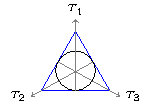
\includegraphics[width=0.48\columnwidth]{dalitz-tri}}
  % 
  \hfill
  % 
  \subbottom[Dalitzplottet med indtegnede resonansbånd. Det smalle røde viser $\alpha_{0}$, mens den bredde
  viser $\alpha_{1}$.]
  {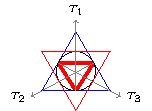
\includegraphics[width=0.48\columnwidth]{dalitz-band}}%
  \caption{}
  \label{fig:dalitz-triangle}
\end{figure}

\subsubsection{Symmetribetragtninger}
\label{sec:symbetragt}

Såfremt der ikke er nogen symmetribegrænsninger og henfaldsprodukterne ikke vekselvirker med
hinanden, vil matrixelementet være en konstant og henfaldet vil udelukkende afgøres af
faserummet. Dette svarer til statistisk henfald og vil give anledning til en flad fordeling
\cite{Fedorov}, hvilket vil være tilfældet ved direkte henfald.

Henfalder systemet i stedet via en resonans for derefter at henfalde til sluttilstanden, vil det ses
på plottet som et bånd. I forhold til den sekventielle henfaldsmodel og koincidensspektrene
forventes bånd svarende til energien af $\alpha_{0}$ og $\alpha_{1}$. Bredden af disse bånd vil være bestemt
af berylliumtilstandens bredde. $\alpha_{1}$-båndet bør derfor være væsentligt breddere, hvilket er
indtegnet på \cref{fig:dalitz-triangle}b. Dalitzplottet kan dermed bruges til at identificere
resonanser og bredden af disse.

$\alpha$-henfaldet er ikke et svagt henfald, så både spin og paritet skal være bevaret. Endvidere er
$\alpha$-partikler bosoner, så den samlede bølgefunktion skal være symmetrisk under ombytning af de tre
$\alpha$-partikler. På baggrund af disse bevarelseslove skal matrixelementet, og dermed Dalitzplottet,
være nul i visse områder. Denne udledning er foretaget i \cite{Fedorov} og resultatet ses på
\cref{fig:dalitz-0}.
%
\begin{figure}[h]
  \centering
  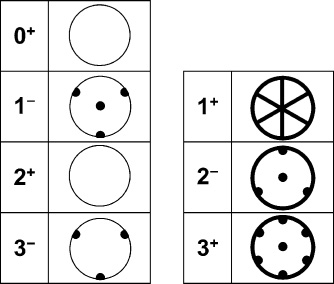
\includegraphics[width=0.3\columnwidth]{dalitz-zero}
  \caption{Områder af Dalitzplottet, hvor fordelingen skal være 0. }
  \label{fig:dalitz-0}
\end{figure}

Den generelle tendens viser, at for tilstandene med unaturlig paritet $\pi = (-1)^{J+1}$, dvs. i højre
kolonne, stiller symmetrien strenge krav til, hvor fordelingen skal være nul. Kravene til
tilstandene med naturlig paritet $\pi = (-1)^{J}$ er væsentligt mindre. Endvidere ses, at det
udelukkende er tilstande med unaturlig paritet, hvor fordelingen skal være nul langs hele randen.

Det er muligt at forklare effekten af $\alpha$-partiklernes bølgenatur på Dalitzplottet mere
intuitivt. Ud fra tre målte energier er der tre mulige måder, hvorpå man kan kombinere de tre
$\alpha$-partikler, således de danner \Be*. Dette svarer til, at der for hver konfiguration er tre
muligheder for hvilken partikel, der udsendes først.

Hvis \Be* tilstanden er smal, er kun en af konfigurationerne realisérbar. Dette svarer til
områderne, hvor $\alpha_{0}$-båndene skærer den indskrevne cirkel på \cref{fig:dalitz-triangle}b. Her er
kun én konfiguration mulig, da den mest energirige partikel nødvendigvis må være
$\alpha_{0}$-partiklen.

% Den første exciterede tilstand i beryllium er dog meget bred, så her vil der være mere end et bidrag
% som summeres. På \cref{fig:dalitz-triangle}b vil det svare til områderne hvor båndene krydser, da
% præcis i disse områder er flere konfigurationsmuligheder.

Den første exciterede tilstand i beryllium er meget bred. I områderne på
\cref{fig:dalitz-triangle}b, hvor $\alpha_{1}$-båndene krydser, vil der være mere end én sandsynlig
konfiguration.  Den endelige bølgefunktion er dermed en linearkombination af flere bølgefunktioner
og idet denne skal være symmetrisk, vil områderne, hvor båndene overlapper, svare til konstruktiv
interferens mellem de enkelte bølgefunktioner. 















\section{Data og databehandling}
\label{sec:dalitz-data}

Databehandlingen af dette er stort set tilsvarende den i \cref{sec:sek-data}. Eneste forskel er, at når
der blev fundet en koincidens, så blev Dalitzkoordinaterne udregnet. Hvis punktet lå uden for den
indskrevne cirkel, så blev det smidt væk.

\subsection{\SI{17.8}{\MeV}}
\label{sec:dalitz-178}


På \cref{fig:dalitz-1077} ses Dalitzplottet for trippel-$\alpha$ henfaldet fra den exciterede tilstand
ved \SI{17.8}{\MeV} i kulstof. %Som forventet er plotet symmetrisk. 

Båndene svarende til $\alpha_{0}$ ses ude ved kanten af cirklen, hvilket stemmer overens med, at de er
det meste energirige partikler i henfaldet. Som forventet er det smalle bånd svarende til at
berylliumresonansen er meget lang livet. Lidt under $\alpha_{0}$ ses også en struktur i dobbeltkoincidenserne,
der ligner lidt en klo. Dette skyldes tilfældige koincidenser, formentlig på grund af beamet. I
Dalitzplottet genfindes også den tidligere observerede tendens med stærk undertrykkelse af $\alpha_{0}$
når dobbeltkoincidenserne benyttes. 

\begin{figure}[t]
  \centering
  \subbottom[Dobbelkoincidenser]{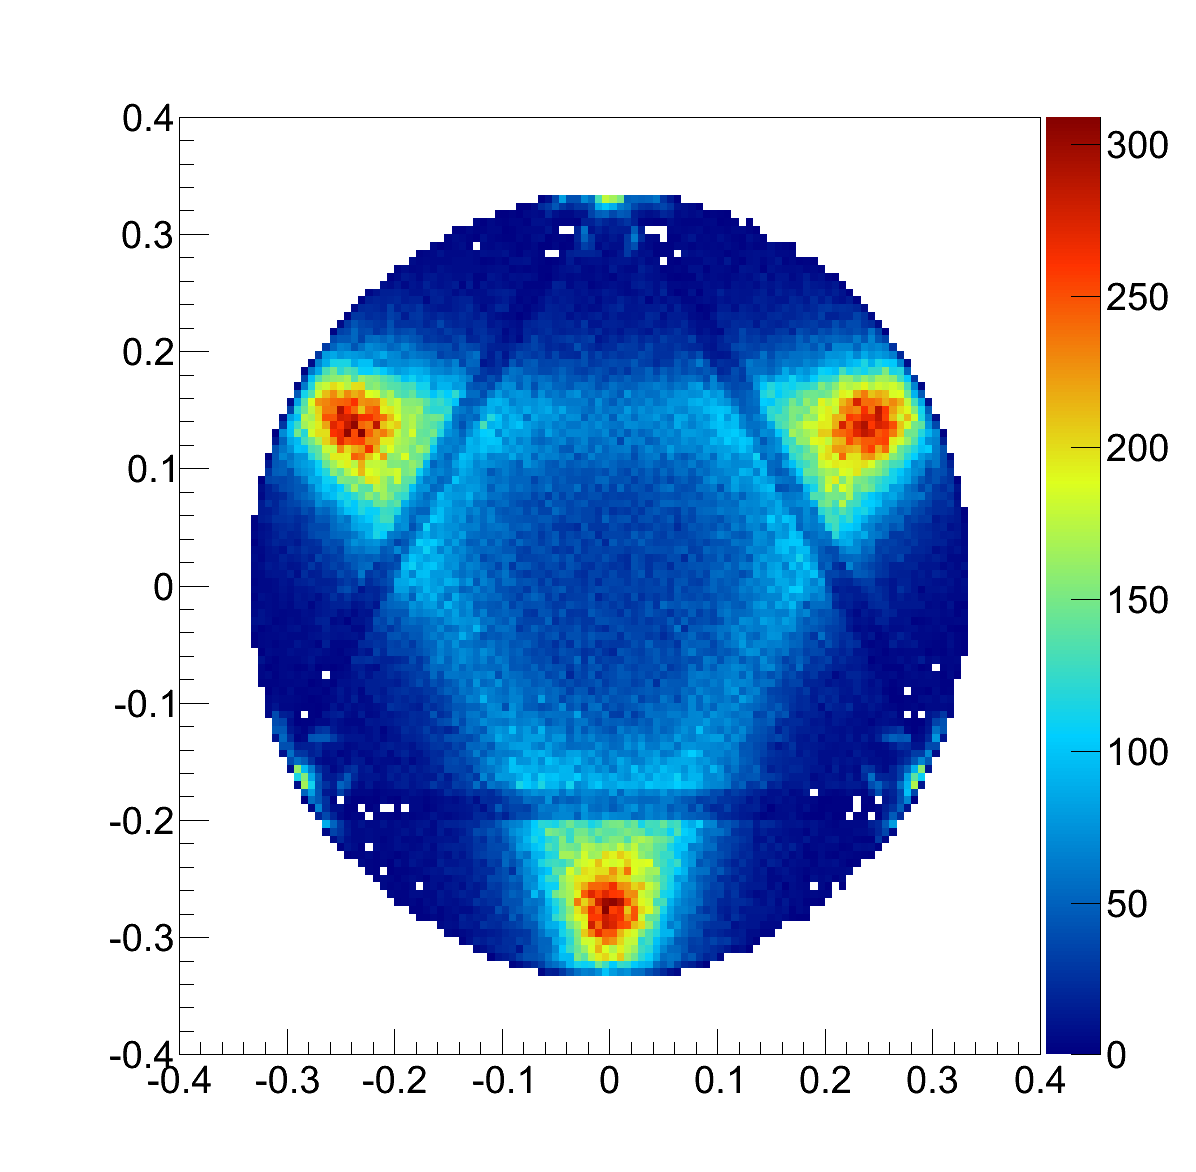
\includegraphics[width=0.46\columnwidth]{1077-Dalitz-D}}%
  \hfill
  \subbottom[Trippelkoincidenser]{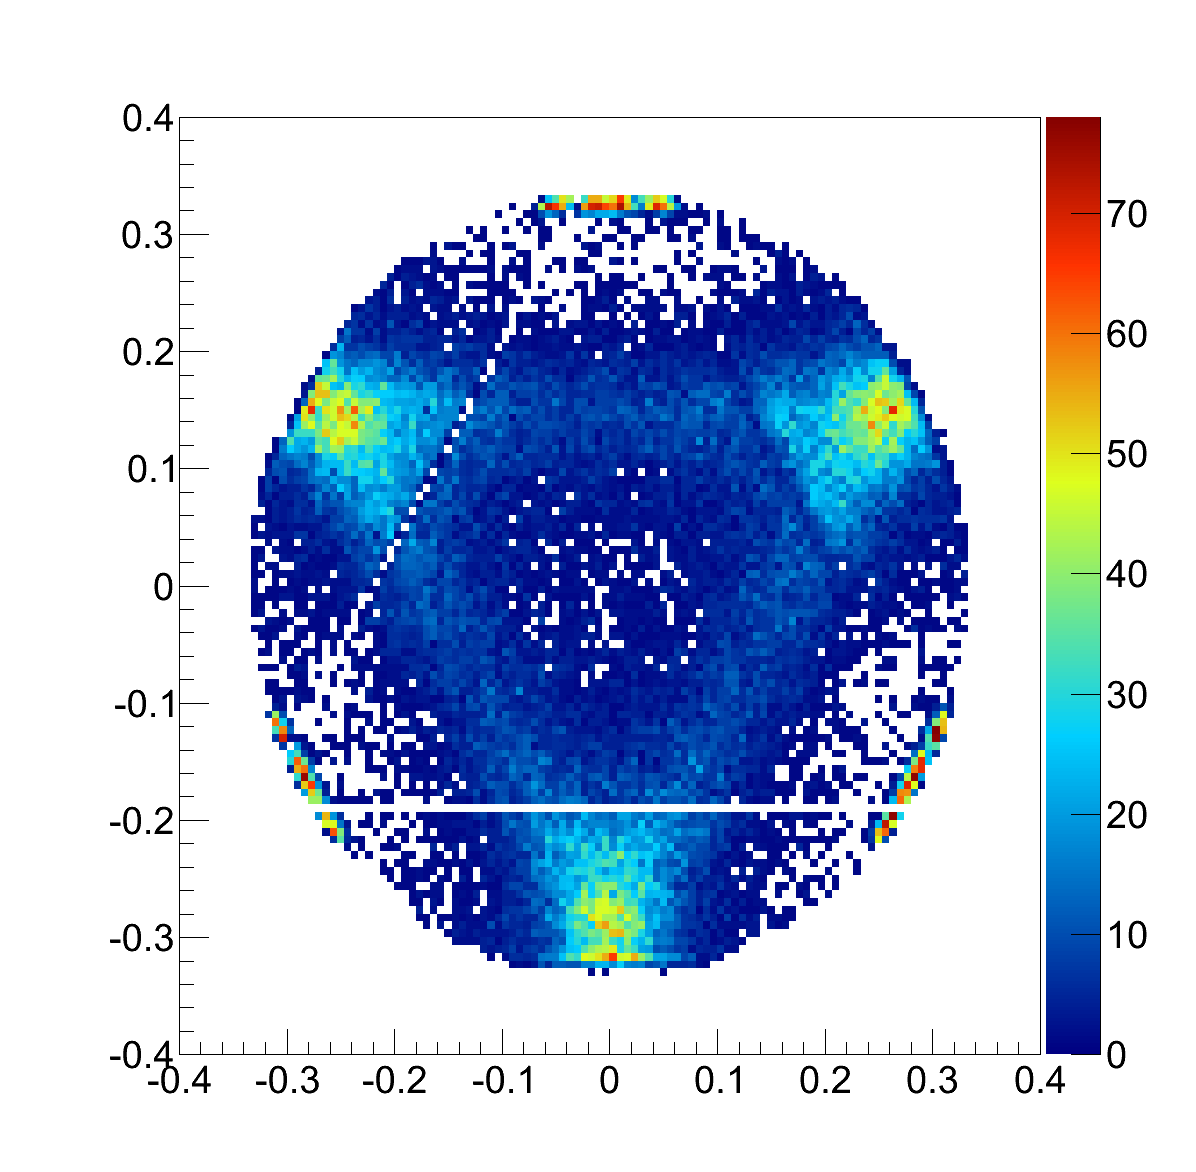
\includegraphics[width=0.46\columnwidth]{1077-Dalitz-T}}%
  \caption{Dalitzplot for $0^{+}$ tilstanden ved \SI{17.8}{\MeV} i kulstof.}
  \label{fig:dalitz-1077}
\end{figure}

Ved lidt lavere energi ses båndene for $\alpha_{1}$. Toppene ude ved sidderne og i bunden har den samme
struktur i de to plots, selv om toppene er mere fremtrædende når dobbeltkoincidenserne
benyttes. Dette skyldes, som tidligere diskuteret, at disse er bedre til at detektere $\alpha_{1}$. I
området mellem toppene er strukturen også den samme. Dobbelkoincidenserne har dog fordelen ved den
øgede datamængde, som får dens strukture til at adskille sig bedre fra baggrunden. Der er dog ingen
tvivl om at bredden af $\alpha_{1}$-båndet er væsentligt større end $\alpha_{0}$-båndet. 

Hvilken tilstand er så blevet populeret? Ud fra \cref{fig:dalitz-0} kan de to tilstande med naturlig
paritet $1^{-}$ og $3^{-}$ udelukkes, da disse kræver, at der er nulpunkter ved de steder
$\alpha_{1}$-båndet har maksima. Alle tilstandene med unaturlig paritet kræver at fordelingen er nul
langs hele randen, hvilket er hvor maksima for både $\alpha_{0}$- og $\alpha_{1}$-båndet befinder sig. Ud over
dette, stiller de også visse andre krav, som ikke heller ikke er opfyldt.

Dermed er antallet af kandidater reduceret til $0^{+}$ og $2^{+}$, for hvilke symmetrien stiller
samme krav. Der er desuden den mulighed, at det kan være en tilstand, som ikke er tabuleret i
\cite{Fedorov}. En videre analyse vil kræve simuleringer, hvilket er uden for tidsrammen af dette
projekt. Heldigvis er tilstanden tabuleret og ifølge \cite{States} er den
populerede tilstand en $0^{+}$ tilstand, hvilket stemmer smukt overens med resultaterne.

















\chapter{Konklusion}
\label{cha:konklusion}


\clearpage
\bibliographystyle{dk-plain-etal}
\bibliography{Bachelor}

\end{document}

%%% Local Variables: 
%%% mode: latex
%%% TeX-engine: default
%%% End: 